% !TeX spellcheck = en_US
\documentclass[12pt]{article}
\usepackage[T1]{fontenc}
\usepackage[utf8]{inputenc}
\usepackage{amsmath,amsthm,amsfonts,amssymb,amscd}
\usepackage[lining,semibold,scaled=1.05]{ebgaramond}     
%\usepackage[cmintegrals,cmbraces]{newtxmath}
% Use FUCKING GARAMOND
\usepackage{hyperref}
\hypersetup{
	colorlinks,
	linkcolor={red!50!black},
	citecolor={blue!50!black},
	urlcolor={blue!80!black}
}
\urlstyle{same}
\usepackage[ebgaramond]{newtxmath}
\usepackage{xparse}
\usepackage{minted}
\usepackage{graphicx}                    
% Publication quality tables          
% Driver-independent color extensions
\usepackage[margin=1in]{geometry}           
% Customize document dimensions        
% all 4 margins to be either 1 inch or 1.5 cm
\usepackage{mathtools}           

% Creating circuits        
% Print exactly what you type in
\usepackage[us]{datetime} 
% Various time format
\usepackage{blindtext}
\usepackage{bbding}
\usepackage[scr=euler,cal=dutchcal,frak=euler,bb=dsfontserif,bbsymbols]{mathalfa}
\usepackage{bbm}
\usepackage{bm}
\usepackage{multirow}
\usepackage{multicol}
\usepackage[x11names,table]{xcolor}
\usepackage[shortlabels]{enumitem}   
\usepackage{standalone}
\usepackage{microtype}
\usepackage{censor}
\usepackage[backend=biber,style=alphabetic]{biblatex}
\usepackage{courier}
\usepackage{movement-arrows}
\usepackage{algorithm}
\usepackage{algpseudocode}
\usepackage[makeroom]{cancel}
\usepackage{tcolorbox}
\tcbuselibrary{skins,raster,theorems,listings,minted}
\usepackage{mathtools}
\usepackage{soul}
\usepackage{multicol}
\usepackage{caption}
\usepackage{wrapfig}
\usepackage{authblk}
\usepackage{float}
\usepackage{fontawesome5}
\usepackage{tikz}
\usetikzlibrary{positioning}
\usetikzlibrary{shapes.geometric,arrows,patterns,arrows.meta, bending,calc,matrix, shadings,intersections,shadows,decorations,fit,backgrounds,circuits.ee.IEC,shapes.callouts}
\newcounter{dummy}



\definecolor{dkgreen}{rgb}{0,0.6,0}
\definecolor{dred}{rgb}{0.545,0,0}
\definecolor{dblue}{rgb}{0,0,0.545}
\definecolor{lgrey}{rgb}{0.9,0.9,0.9}
\definecolor{gray}{rgb}{0.4,0.4,0.4}
\definecolor{darkblue}{rgb}{0.0,0.0,0.6}
\DeclareMathOperator*{\argmax}{arg\,max}
\DeclareMathOperator*{\argmin}{arg\,min}


\renewcommand{\labelitemi}{$\textcolor{SteelBlue4}{\bullet}$}
\renewcommand{\labelitemii}{$\textcolor{blue}{\cdot}$}
\renewcommand{\labelitemiii}{$\textcolor{SkyBlue4}{\diamond}$}
\renewcommand{\labelitemiv}{$\textcolor{SkyBlue4}{\ast}$}

\newcommand{\enf}[1]{\textcolor{DodgerBlue3}{\textbf{#1}}} %enf sta per enfasi
\let\emph\enf
\newcommand{\sott}[1]{\setulcolor{SkyBlue3}\ul{#1}}
\let\underline\sott

\newcommand{\prob}{\mathbb{P}}
\newcommand\independent{\protect\mathpalette{\protect\independenT}{\perp}}
\newcommand{\ev}{\mathbb{E}}
\def\independenT#1#2{\mathrel{\rlap{$#1#2$}\mkern2mu{#1#2}}}
\newcommand{\Z}{\mathbb{Z}}
\newcommand{\R}{\mathbb{R}}
\newcommand{\N}{\mathbb{N}}
\newcommand{\T}{\mathbb{T}}
\newcommand{\Tbar}{\overline{\T}}
\newcommand{\A}{\mathscr{A}}
\newcommand{\Nstar}{\N^{*}}
\newcommand{\Rext}{\overline{\R}}
\newcommand{\io}{\text{ i.o.}}
\newcommand{\normale}{\mathcal{N}}
\newcommand{\equalexpl}[1]{%
	\underset{\substack{\uparrow\\\mathrlap{\text{\vspace{-3cm}\hspace{-1em}#1}}}}{=}}
\newcommand{\dif}{\mathop{}\!\mathrm{d}}
\newcommand{\convas}{\xrightarrow[]{\text{a.s.}}}
\newcommand{\convpr}{\xrightarrow[]{\pr}}
\newcommand{\convd}{\xrightarrow[]{\text{d}}}
\newcommand{\convlp}{\xrightarrow[]{\lp}}
\newcommand{\lone}{L^{1}}
\newcommand{\convw}{\xrightarrow[]{\mathrm{weak}}}
\newcommand{\as}{\text{ a.s.}}
\newcommand{\asstnr}{\sim N(0,1)}
%\def\checkmark{\tikz\fill[scale=0.4](0,.35) -- (.25,0) -- (1,.7) -- (.25,.15) -- cycle;} 
\newcommand{\dx}{\dif x}
\newcommand{\dy}{\dif y}
\newcommand{\dt}{\dif t}
\newcommand{\du}{\dif u}
\newcommand{\ds}{\dif s}
\newcommand{\dw}{\dif\omega}
\newcommand{\dz}{\dif z}
\newcommand{\dmu}{\dif\mu}
\newcommand{\dpr}{\dif\pr}
\newcommand{\E}{\mathscr{E}}
\newcommand{\B}{\mathscr{B}}
\newcommand{\F}{\mathscr{F}}
\newcommand{\G}{\mathscr{G}}
\newcommand{\HS}{\mathscr{H}}
\newcommand{\Zn}{\mathscr{Z}}
\newcommand{\D}{\mathscr{D}}
\newcommand{\xbar}{\overline{X}}
\newcommand{\rbar}{\overline{\R}}
\newcommand{\ybar}{\overline{Y}}
\newcommand{\xxbar}{\overline{\xbar}}
\newcommand{\xtilde}{\widetilde{X}}
\newcommand{\ifonly}{\underline{if and only if}}
\newcommand{\ang}[1]{\langle#1\rangle}

\newcommand{\ubracketthin}[1]{\underbracket[0.3pt]{#1}}

\newcommand*\circled[1]{\tikz[baseline=(char.base)]{
		\node[shape=circle,draw,
		shading=ball, ball color=SkyBlue1!70,
		,inner sep=1.5pt] (char) {\scriptsize\bfseries #1};}}
\newcommand{\circnum}{\protect\circled{\arabic*}}
\newcommand{\circlet}{\protect\circled{\alph*}}	
\newcommand{\bbg}[1]{%
	\ooalign{$#1$\cr\raisebox{-.2pt}{$#1$}\cr\raisebox{.2pt}{$#1$}\cr\textcolor{white}{$\mkern0.2mu#1$}}%
}
\newcommand{\leb}{\bbg{\lambda}}

%i comandi di MERDA di stefano
\newcommand{\ra}{\rightarrow}
\newcommand{\iy}{\infty}
\newcommand{\mE}{\mathbb{E}}
\newcommand{\mP}{\mathbb{P}}
\newcommand{\mB}{\mathcal{B}(\mathbb{R})}
\newcommand{\mL}{\mathbb{L}}
\newcommand{\ninfty}{n\to$\infty$}
\newcommand{\tinfty}{t\to$\infty$}
\newcommand{\xinfty}{x\to$\infty$}
\newcommand{\yinfty}{y\to$\infty$}
\newcommand{\mLL}{\mathbb{L}^2(0,T)}
\newcommand{\mR}{\mathbb{R}}
\newcommand{\mC}{\mathcal{C}}
\newcommand{\mRd}{\mathbb{R}^d}
\newcommand{\mN}{\mathbb{N}}
%\newcommand{\m1}{\mathbf{1}}
\newcommand{\mF}{\mathcal{F}}
\newcommand{\mM}{\mathcal{M}}
\newcommand{\mW}{\mathcal{W}}
\newcommand{\mV}{\mathcal{V}}
\newcommand{\mA}{\mathcal{A}}
\newcommand{\mez}{\frac{1}{2}}
\newcommand{\intT}{\int_{0}^{T}}
\newcommand{\nN}{n \in \mathbb{N}}
\newcommand{\mmN}{\mathcal{N}}
\newcommand{\BM}{(B_t)_{t\geq 0}}
\newcommand{\PX}{(X_t)_{t\geq 0}}
\newcommand{\var}{\mathbb{V}\!\mathrm{ar}\,}
\newcommand{\cov}{\mathbb{C}\mathrm{ov}\,}
\newcommand{\lp}{L^{p}}
\newcommand{\BMF}{\left((B_t)_{t\geq 0},\mathcal{F}_t \right)}
\newcommand{\mFt}{\mathcal{F}_t}
\newcommand{\every}{\forall\,}
\newcommand{\dyadic}{\mathcal{d}}
\newcommand{\norm}[1]{\left|\negthinspace\left|#1\right|\negthinspace\right|}
\newcommand{\pr}{\mathbb{P}}
\newcommand{\indi}{\mathbb{1}}
\newcommand{\trns}[1]{{#1}^{\scriptscriptstyle\mathsf{T}}}
\newcommand{\iid}{\stackrel{\mathrm{iid}}{\sim}}
\newcommand{\unmezz}{\frac{1}{2}}
\newcommand{\sa}{$\sigma$-algebra}	\newcommand{\rv}{random variable}
\newcommand{\prefacename}{Preface}
\newcommand{\cinlar}{Çinlar }
\newenvironment{preface}{
	\vspace*{\stretch{2}}
	{\noindent \bfseries \huge\color{SkyBlue4} \prefacename}
	\begin{center}
		% \phantomsection \addcontentsline{toc}{chapter}{\prefacename} % enable this if you want to put the preface in the table of contents
		\thispagestyle{plain}
	\end{center}%
}
{\vspace*{\stretch{5}}}


\newenvironment{closethedeal}{
	\vspace*{\stretch{2}}
	{\noindent \bfseries \huge\color{SkyBlue4} That's all, folks}
	\begin{center}
		% \phantomsection \addcontentsline{toc}{chapter}{\prefacename} % enable this if you want to put the preface in the table of contents
		\thispagestyle{plain}
	\end{center}%
}
{\vspace*{\stretch{5}}}
\pgfkeys{%
	/calloutquote/.cd,
	width/.code                   =  {\def\calloutquotewidth{#1}},
	position/.code                =  {\def\calloutquotepos{#1}}, 
	author/.code                  =  {\def\calloutquoteauthor{#1}},
	/calloutquote/.unknown/.code   =  {\let\searchname=\pgfkeyscurrentname
		\pgfkeysalso{\searchname/.try=#1,                                
			/tikz/\searchname/.retry=#1},\pgfkeysalso{\searchname/.try=#1,
			/pgf/\searchname/.retry=#1}}
}  


\newcommand\calloutquote[2][]{%
	\pgfkeys{/calloutquote/.cd,
		width               = 5cm,
		position            = {(0,-1)},
		author              = {}}
	\pgfqkeys{/calloutquote}{#1}                   
	\node [rectangle callout,draw,callout relative pointer={\calloutquotepos},text width=\calloutquotewidth,/calloutquote/.cd,
	#1] (tmpcall) at (0,0) {#2};
	\node at (tmpcall.pointer){\calloutquoteauthor};    
}  		


\newcommand\lemmethink[2][]{%
	\pgfkeys{/calloutquote/.cd,
		width               = 5cm,
		position            = {(0,-1)},
		author              = {}}
	\pgfqkeys{/calloutquote}{#1}                   
	\node [cloud callout,draw,callout relative pointer={\calloutquotepos},text width=\calloutquotewidth,/calloutquote/.cd,
	#1] (tmpcall) at (0,0) {#2};
	\node at (tmpcall.pointer){\calloutquoteauthor};    
}  											


\renewcommand\leq\leqslant
\renewcommand\geq\geqslant		
\setlength\parindent{0pt}

%%%%%%%%%%%%%%%%%%%%%%%%%%%%%%%%%%%%%%%%%%%%%%%%%%%%%%%%%%%%%%
%%%%%%%%%%%%%%%%%%%%%%%%%%%%%%%%%%%%%%%%%%%%%%%%%%%%%%%%%%%%%%
\usemintedstyle{monokai}
\definecolor{codeBg}{HTML}{282822}
\newenvironment{py}
{\VerbatimEnvironment
	\begin{minted}[
		bgcolor=codeBg,
		breaklines,
		fontsize=\footnotesize
		]
		{python}}
	{\end{minted}}

	%\newmintinline[bluecode]{c++}{\color{codeblue}}
	
\newcommand{\pyinl}[1]{\mintinline[bgcolor=black!40]{python}{#1}}
%%%%%%%%%%%%%%%%%%%%%%%%%%%%%%%%%%%%%%%%%%%%%%%%%%%%%%%%%%%%%%

%%%%%%%%%%%%%%%%%%%%%%%%%%%%%%%%%%%%%%%%%%%%%%%%%%%%%%%%%%%%%%%
\definecolor{UM_Brown}{HTML}{3D190D}
\definecolor{UM_DarkBlue}{HTML}{2264B0}
\definecolor{UM_LightBlue}{HTML}{1CA9E1}
\definecolor{UM_Orange}{HTML}{fEB415}
\addbibresource{biblio.bib}




\setminted{style=monokai}
\usepackage{pygmentex}
\tikzstyle{startstop} = [rectangle, rounded corners, minimum width=3cm, minimum height=1cm,text centered, draw=black, fill=red!30]
\tikzstyle{io} = [trapezium, trapezium left angle=70, trapezium right angle=110, minimum width=3cm, minimum height=1cm, text centered, draw=black, fill=blue!30]
\tikzstyle{process} = [rectangle, minimum width=3cm, minimum height=1cm, text centered, draw=black, fill=orange!30]
\tikzstyle{decision} = [diamond, minimum width=3cm, minimum height=1cm, text centered, draw=black, fill=green!30]
\tikzstyle{arrow} = [thick,->,>=stealth]

\begin{document}
	\textcolor{UM_Brown}{
		\begin{center}
			\textbf{\Large Simulations}\\
			\vspace{5pt}
			Homework 7 \\
			\vspace{5pt}
			\textbf{M.S. in Stochastics and Data Science}\\
			\vspace{20pt}
			\textit{Andrea Crusi, Lorenzo Sala} \\
			\vspace{5pt}
			\today
		\end{center}
		\vspace{10pt}
		\hrule
	}
	
	
	
	
	%%%%%%%%%%%%%%% NEW SECTION %%%%%%%%%%%%%%% 
	\section{Exercise 1}
	\subsection{Overview}
	We start this discussion by taking a look at the main characteristics of the network of queues in question.\\
	In this system we have $N=10$ machines departing from the ``delay station'' $Z$ with a certain rate (which is modeled by a random variable $Z$); from here they reach a short repair station where they undergo a short reparation whose duration is another random variable $X$; finally, with a probability $\beta=0.2$ they reach a long repair station where the duration of the repair is yet another random variable $Y$. The machines that do not go the the long repair station or that have finished the long repair go back to the source.
	In this case the distribution of all the three stations is \emph{negative exponential distributions}:
	\begin{equation*}
		F_X(x)=\pr(X\leq x)=1-e^{-\frac{1}{\eta} x}\qquad f_X(x)=\frac{\dif F_X}{\dx}=\lambda e^{-\frac{1}{\eta} x}.
	\end{equation*}
	In this formulation the parameter is given directly as the expected value $\ev[X]=\eta$ of the distribution. We have our three expected values, reflecting the average time of each of these three events:
	\begin{enumerate}[\circnum]
		\item time between breakages of a machine: $\eta_{\mathsf{arrival}}=3000\text{ mins}$;
		\item service time of the short repair station: $\eta_{\mathsf{short}}=40\text{ mins}$;
		\item service time of the long repair station: $\eta_{\mathsf{long}}=960\text{ mins}$.
	\end{enumerate}
	This characteristic brings us to the particular case of the tandem server with ``M/M/2'' service and arrival times seen during lectures. 
In this scenario, due to the memoryless property of the negative exponential distribution for all time variables (e.g., failure times, short and long repair times), defining regeneration points is straightforward. For example, a regeneration point can be set as the time when a machine enters the long repair station and the system resets to its initial conditions. This choice is based on the following schema:
		
		\begin{table}[H]
			\centering
			\renewcommand{\arraystretch}{1.5}
			\begin{tabular}{|m{4cm}|m{4cm}|m{4cm}|}
				\hline
				\multicolumn{1}{|c|}{\textbf{Service time distribution of the first queue}} &
				\multicolumn{2}{c|}{\textbf{Service time distribution of the second queue}} \\ 
				\cline{2-3}
				& \textbf{GENERIC} & \textbf{MARKOV (Neg-Exp)} \\ 
				\hline
				\textbf{GENERIC} & Any departure that leaves behind exactly $N - 1$ customers from one of the two servers of the network & Any departure from the first server \\ 
				\hline
				\textbf{MARKOV (Neg-Exp)} & Any departure from the second server & Any departure in the system \\ 
				\hline
			\end{tabular}
			\caption{Service time distribution schema for the first and second queue.}
		\end{table}
	in which we can easily notice we are in the bottom-right case, in which the service times of both the queue are negative-exponential.\\
	Technically every departure could be a regeneration point but since our analysis focuses on the average waiting time of the long repair station we chose as regeneration points all the departures from the long station. 
	This choice will also simplify our calculations: the value $\nu_{j}$, that counts the number of the occurrences of the event of interest in the current regeneration cycle, will always be 1. \\
	For the distribution of the routings we assume a uniform distribution (so that 20\% of the departures from the short station will become an arrival to the long station).
	\subsection{The simulation}
	For the implementation of this simulation we chose the classic event list approach: the bulk of the simulator is an ever-growing list of events sorted by the timestamp of their occurrence. Each of these events is ``processed'' one by one, typically by adding another related event to the list and computing the necessary measurements. \\
	\begin{figure}[h]
		\centering
			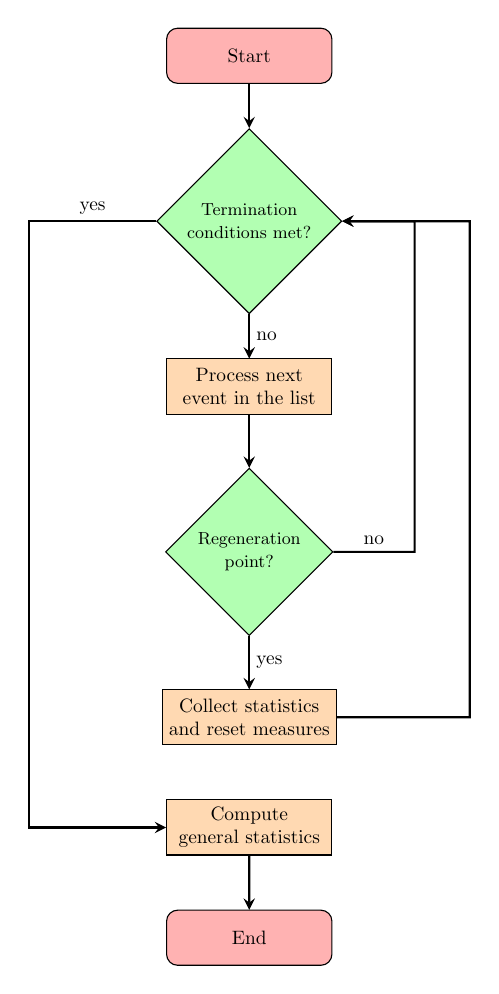
\begin{tikzpicture}[scale=0.7, every node/.style={scale=0.7},node distance=2cm]
			\node (start) [startstop] {Start};
			\node (conditions) [decision, align=center, below of=start,yshift=-1cm] {\small Termination \\ \small conditions met?};
			\node (mainloop) [process,below of=conditions,yshift=-1cm,align=center] {Process next \\ event in the list};
			\node (regen) [decision, align=center, below of=mainloop,yshift=-1cm] {\small Regeneration\\ \small point?};
			\node (collect) [process, below of=regen, yshift=-1cm,align=center]{Collect statistics \\ and reset measures};
			\node (terminate) [process, below of=collect,align=center]{Compute\\ general statistics};
			\node (end) [startstop,below of=terminate] {End};
			\draw [arrow] (start)--(conditions);
			\draw [arrow] (conditions)--node[anchor=south]{yes}+(-4,0)|- (terminate);
			\draw [arrow] (conditions)--node[anchor=west]{no}(mainloop);
			\draw[arrow] (mainloop)--(regen);
			\draw[arrow] (regen)--node[anchor=west]{yes}(collect);
			\draw[arrow] (regen)--node[anchor=south]{no}+(3,0)|-(conditions);
			\draw[arrow](collect)--+(4,0)|-(conditions);
			\draw[arrow](terminate)--(end);
		\end{tikzpicture}
	\end{figure}

	\section*{Simulation Results for 10 Customers}
	The simulation gives the following results:
	
	\noindent\textbf{Station 0 Results:}
	\begin{table}[h!]
		\centering
		\begin{tabular}{@{}l l@{}}
			\toprule
			Throughput ($X[10]$)              & \textbf{0.002935} \\
			Utilization ($U[10]$)             & \textbf{0.880562} \\
			Mean queue length ($n[10]$)       & \textbf{8.805621} \\
			Mean waiting time ($w[10]$)       & \textbf{3000.000000} \\
			Mean response time ($R_0$)        & \textbf{406.914799} \\
			\bottomrule
		\end{tabular}
	\end{table}
	
	\noindent\textbf{Station 1 Results:}
	\begin{table}[h!]
		\centering
		\begin{tabular}{@{}l l@{}}
			\toprule
			Throughput ($X[10]$)              & \textbf{0.002935} \\
			Utilization ($U[10]$)             & \textbf{0.117408} \\
			Mean queue length ($n[10]$)       & \textbf{0.131229} \\
			Mean waiting time ($w[10]$)       & \textbf{44.708658} \\
			Mean response time ($R_0$)        & \textbf{84.708658} \\
			\bottomrule
		\end{tabular}
	\end{table}
	
	\noindent\textbf{Station 2 Results:}
	\begin{table}[h!]
		\centering
		\begin{tabular}{@{}l l@{}}
			\toprule
			Throughput ($X[10]$)              & \textbf{0.000587} \\
			Utilization ($U[10]$)             & \textbf{0.563560} \\
			Mean queue length ($n[10]$)       & \textbf{1.063150} \\
			Mean waiting time ($w[10]$)       & \textbf{1811.030708} \\
			Mean response time ($R_0$)        & \textbf{2771.030708} \\
			\bottomrule
		\end{tabular}
	\end{table}
	
	
	we can notice easily that the mean waiting time for the long repair station is $1811.030$ which is compatible with our benchmark. 
	
	\section{Exercise 2}
	The second exercise focuses on analyzing the Machine Repairman system under a modified scenario where the repair time for machines directed to the long repair lab is modeled using a hyper-exponential distribution. This distribution introduces two exponential phases, reflecting high variability in repair durations, and is defined by the following parameters:
	
	\begin{itemize}
		\item \textbf{Phase 1:} Weight $\alpha_1 = 0.95$, Mean $\mu_1 = 10$ minutes.
		\item \textbf{Phase 2:} Weight $\alpha_2 = 0.05$, Mean $\mu_2 = 19010$ minutes.
	\end{itemize}
	
	This configuration captures the reality of repair processes, where most failures are resolved quickly, but a small fraction requires significantly longer times.
	
	The objective is to estimate the average waiting time at the long repair station using the regenerative simulation method. The analysis must achieve a confidence level of $95\%$ and ensure the width of the confidence interval is no greater than $10\%$ of the point estimate. Validation of the simulation model is incorporated by introducing a modification that enables the system to be solved analytically using the Mean Value Analysis algorithm. This allows for a comparison between simulated and analytical results, ensuring the reliability and accuracy of the findings.
	
	In order to solve this exercise we have, firstly, to give a look to the table shown above, here we are in the bottom-left part, since the first queue is negative-exponential, while the second is not. Hence, we can choose again the departure from the long-repair station as a regenerating point.
	
	
\end{document}
